\documentclass{article}

% if you need to pass options to natbib, use, e.g.:
% \PassOptionsToPackage{numbers, compress}{natbib}
% before loading nips_2017
%
% to avoid loading the natbib package, add option nonatbib:
% \usepackage[nonatbib]{nips_2017}

\usepackage{graphicx}
\usepackage{nips_2017}

% to compile a camera-ready version, add the [final] option, e.g.:
% \usepackage[final]{nips_2017}

\usepackage[utf8]{inputenc} % allow utf-8 input
\usepackage[T1]{fontenc}    % use 8-bit T1 fonts
\usepackage{hyperref}       % hyperlinks
\usepackage{url}            % simple URL typesetting
\usepackage{booktabs}       % professional-quality tables
\usepackage{amsfonts}       % blackboard math symbols
\usepackage{nicefrac}       % compact symbols for 1/2, etc.
\usepackage{microtype}      % microtypography

\title{Detecting Credit Card Fraud in a Skewed Data Set Using Deep Learning}

% The \author macro works with any number of authors. There are two
% commands used to separate the names and addresses of multiple
% authors: \And and \AND.
%
% Using \And between authors leaves it to LaTeX to determine where to
% break the lines. Using \AND forces a line break at that point. So,
% if LaTeX puts 3 of 4 authors names on the first line, and the last
% on the second line, try using \AND instead of \And before the third
% author name.

\author{
  Isaac Smith \\
  Department of Computer Science\\
  South Dakota School of Mines & Technology\\
  Rapid City, SD 57110 \\
  %% examples of more authors
  %% \And
  %% Coauthor \\
  %% Affiliation \\
  %% Address \\
  %% \texttt{email} \\
  %% \AND
  %% Coauthor \\
  %% Affiliation \\
  %% Address \\
  %% \texttt{email} \\
  %% \And
  %% Coauthor \\
  %% Affiliation \\
  %% Address \\
  %% \texttt{email} \\
  %% \And
  %% Coauthor \\
  %% Affiliation \\
  %% Address \\
  %% \texttt{email} \\
}

\begin{document}
% \nipsfinalcopy is no longer used

\maketitle

\begin{abstract}
 [PUT THE ABSTRACT HERE WHEN YOU'RE DONE]
\end{abstract}

\section{Introduction}

 Credit card fraud is a problem for many people across the United States,
 with 45,428 cases of credit card fraud reported to the Federal Trade Commission in 2017.
 With datasets available today, neural networks can be trained to identify trends
 in fraudulent and non-fraudulent transactions.

 The output of these networks can be used to notify consumers of
 suspicious activity on their accounts and prevent further losses.


\subsection{The Dataset}


For this case study, the dataset consists of over 280,000 credit card transaction 
data points accumulated over 2 days in European countries\footnote{Dataset from
 https://www.kaggle.com/mlg-ulb/creditcardfraud.}. Each data point 
holds basic information about the transaction as well as obfuscated data resulting 
from a PCA transformation, which can be seen in Table~\ref{sample-points} . The data 
prefixed with a “V” is the transformed data.

\begin{table}[htb]
  \caption{Sample Transaction Data Points}
  \label{sample-points}
  \centering
  \begin{tabular}{llllllll}	
    \toprule
    Time & V1 & V2  & ... & V27 & V28 & Amount & Class \\
    \midrule
    0 & -1.359807134  & -0.072781173 &    ...    & 0.133558377 & -0.021053053 & 149.62 & 0    \\
    70071 & -0.440095203  & 1.137238976 &    ...    & 0.768290751 & 0.459623328 & 227.3 & 1    \\
    132086 & -0.361427839 & 1.133471917 &    ...    & -0.001249817 & -0.182750897 & 480.72 & 1 \\
    150426 & -0.269118964  & -0.063708356 &    ...    & 0.385434237 & 0.21311729 & 7.33 & 0    \\
    172792 & -0.533412522  & -0.189733337 &    ...    & -0.002415309 & 0.013648914 & 217 & 0    \\
    \bottomrule
  \end{tabular}
\end{table}

 One of the interesting metrics of the dataset is the ratio of fraudulent to non-fraudulent transactions. 
 With fraudulent transactions only making up 0.172\% of the 280,000+ transactions, this poses a 
 challenge for a neural to make accurate identifications for fraudulent cases. 

\begin{figure}
  \begin{center}
    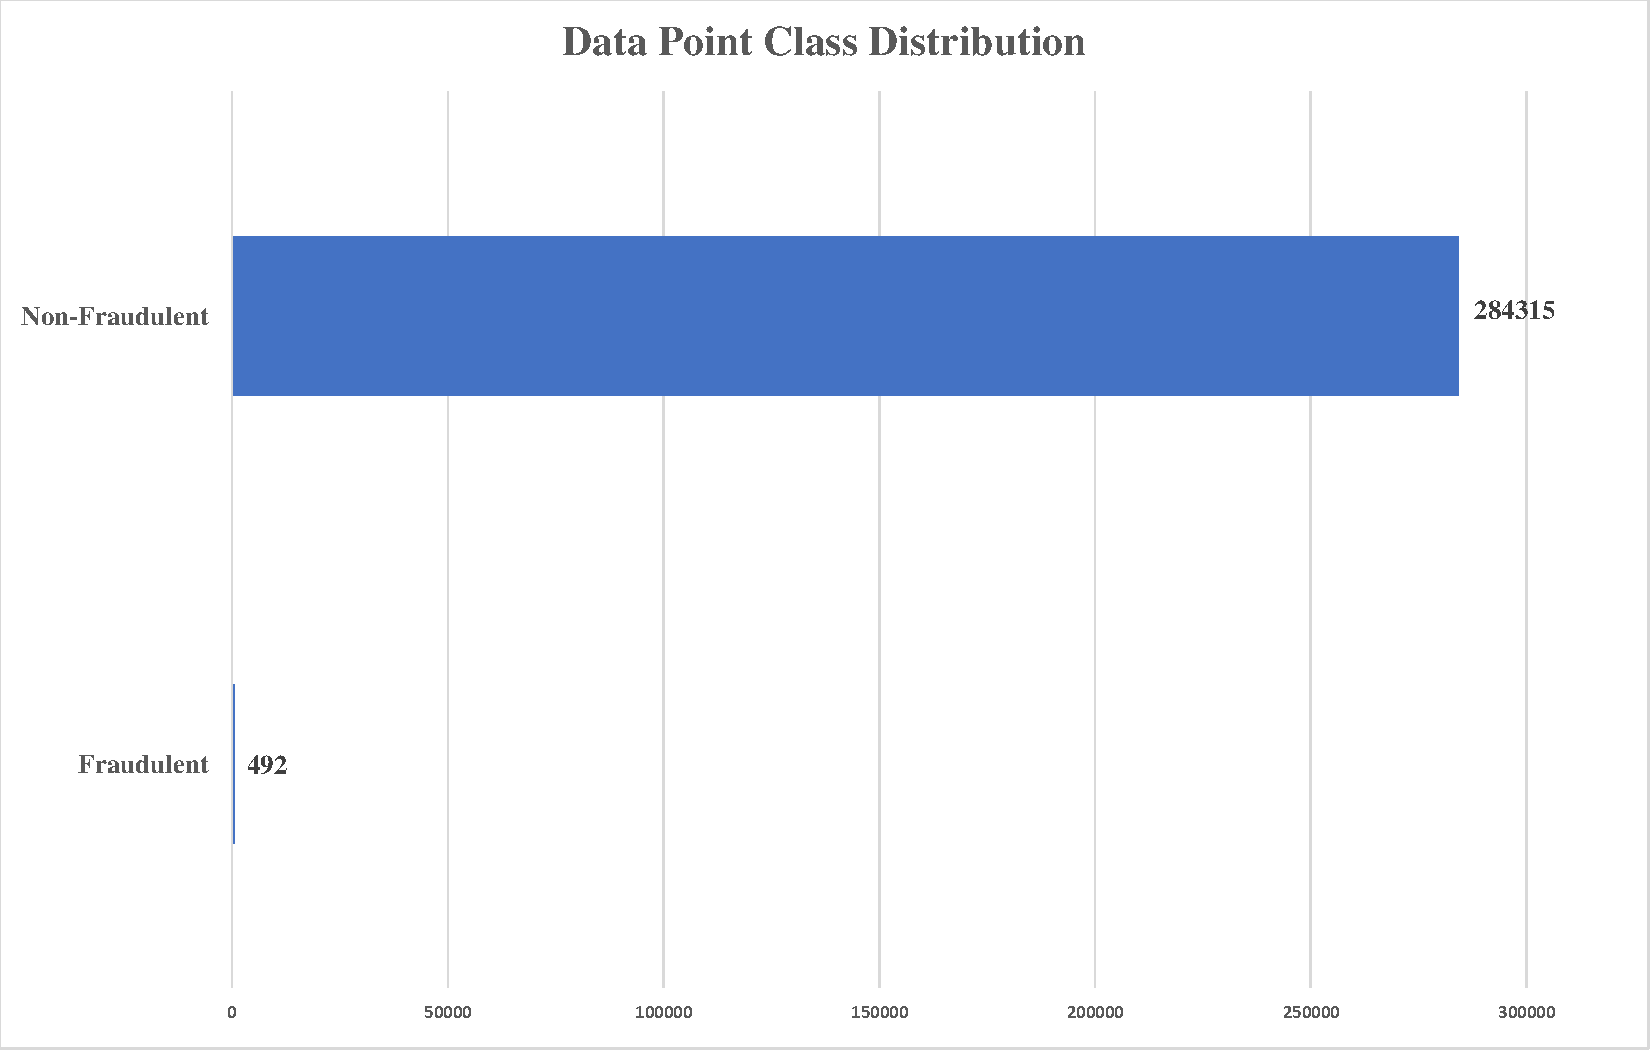
\includegraphics[width=100mm]{DataDistribution.pdf}
    \caption{Distribution between fraudulent and non-fraudulent data points.}
    \label{data-distribution}
  \end{center}
\end{figure}

 The fraudulent cases are also the most interesting result from the network, as simply identifying the 
 99.82800\% of non-fraudulent cases is trivial. The skewed distribution of data points is illustrated
 in Figure~\ref{data-distribution}


\section{Methods}


\subsection{Deep Learning Framework}

 TensorFlow r1.8 was used to carry the back end of the neural network, providing definitions
 for layers, optimization functions, back propagation, and running of the network. The Pandas 
 package was used heavily for the data pre-processing and matrix manipulations.

\subsection{Data Pre-Processing}

 The dataset is provided in a .csv format, so the first pre-processing step is to read the data points 
 into the Pandas package. Once the data is read in, the “Class” property is changed into two properties,
 named “Fraud” and “NonFraud” for easier determination of the output of the network. The fraudulent 
 and non-fraudulent cases are then split into two lists for division of training and testing data. 75\% 
 of each case is used as training data, while the remaining  25\% is used for testing data. Both the 
 training and test data are further divided into various targeted lists for result processing later in the network.

\subsubsection{Augmentation of Fraudulent Cases}

 To overcome the skewed nature of the dataset, augmentation of the fraudulent cases is required. 
 Augmentation was accomplished by sampling the fraudulent cases in both the training and testing sets 600 times, 
 to obtain a ratio between the cases of around 50:50.


\subsection{Neural Network Architecture}

\begin{figure}
  \begin{center}
    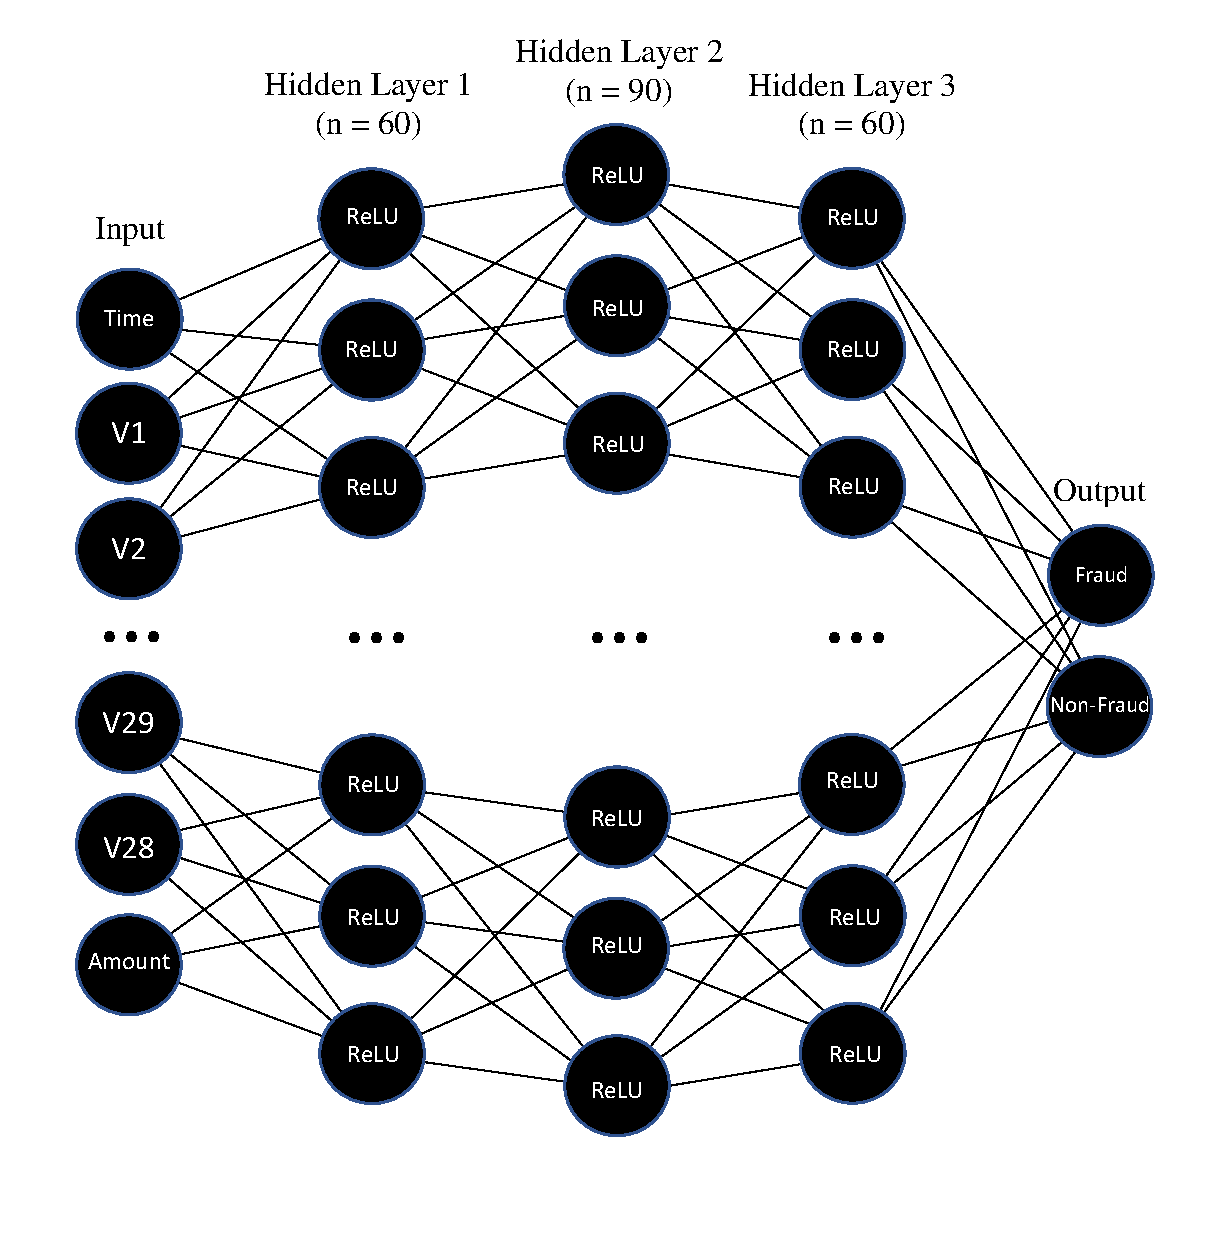
\includegraphics[width=100mm]{NeuralNetDiagramPDF.pdf}
    \caption{Diagram of neural network architecture.}
    \label{network-architecture}
  \end{center}
\end{figure}

 \subsubsection{Layer Definitions}

 The neural network is defined by an input layer, three hidden layers, and an output layer, as can 
 be seen in Figure~\ref{network-architecture}. Each layer also includes a bias input. The input layer is the 
 width of each data point (30), with each layer doubling the width of the previous layer until the 
 output layer, which is of width 2. A fully connected network approach is also used.

\subsubsection{Weight and Bias Initializations}

 Each layer’s weights are initialized using a random generated number from a normal distribution 
 with a standard deviation of  0.1 and centered around zero. The bias weights are initialized in a 
 similar fashion.

\subsubsection{Activation Functions}

 Activation functions used between layers are rectified linear units (RELU), as well as a linear 
 activation function leading to the output layer.

\subsubsection{Output Interpretation}

 The cost function used for interpretation of the network output is mean squared error (MSE). 
 The accuracy of the output is determined by selecting the index of the output node with higher 
 activation and comparing it to index of the output node of the expected result.

\section*{References}

References follow the acknowledgments. Use unnumbered first-level
heading for the references. Any choice of citation style is acceptable
as long as you are consistent. It is permissible to reduce the font
size to \verb+small+ (9 point) when listing the references. {\bf
  Remember that you can go over 8 pages as long as the subsequent ones contain
  \emph{only} cited references.}
\medskip

\small

[1] Alexander, J.A.\ \& Mozer, M.C.\ (1995) Template-based algorithms
for connectionist rule extraction. In G.\ Tesauro, D.S.\ Touretzky and
T.K.\ Leen (eds.), {\it Advances in Neural Information Processing
  Systems 7}, pp.\ 609--616. Cambridge, MA: MIT Press.

[2] Bower, J.M.\ \& Beeman, D.\ (1995) {\it The Book of GENESIS:
  Exploring Realistic Neural Models with the GEneral NEural SImulation
  System.}  New York: TELOS/Springer--Verlag.

[3] Hasselmo, M.E., Schnell, E.\ \& Barkai, E.\ (1995) Dynamics of
learning and recall at excitatory recurrent synapses and cholinergic
modulation in rat hippocampal region CA3. {\it Journal of
  Neuroscience} {\bf 15}(7):5249-5262.

\end{document}
